\documentclass{article}
\usepackage[utf8]{inputenc}

\title{CS63 Final Project}
\author{dhawkin1}
\date{December 2022}

\documentclass[11pt]{article}
\usepackage{fullpage}
\usepackage{graphicx}
\usepackage{wrapfig}


\title{CS63 Spring 2022\\Using a Neural Network to Recognise type of Flowers}
\author{Delaney Hawkins, Yael Borger}
\date{}

\begin{document}

\maketitle

\section{Introduction}

%Your paper should be 4-6 pages long.  In this section you should give

%a broad introduction to your project.  Assume that you are writing to
%an audience that is familiar with AI, but may not know the details of
%the particular technique that you are using.  You should give an
%overview of the approach being explored, and how you applied it to a
%particular problem. 

For this project we will be using a Neural Network to determine if an image containing a flower is a daisy, dandelion, rose, sunflower, or tulip. We will specifically be using a neural network made with many layers of varying types to create specialized feature detectors that are able to recognise key aspects of each type of flower so that it can be labeled appropriately. 


\section{Methods}

We sourced our data set from Kaggle. The data set contained 764 daisy images, 1052 dandelion images, 784 rose images, 733 sunflower images,and 984 tulip images, all in folder labeled with the flowers. 
The data set contained a wide variety of flower images including black and white images, drawings of flowers, images in which only part of the flower was visible, images where the flower was obstructed by bugs, people holding flowers and some images that were seemingly included by accident without visible flowers in them. After they were imported we assigned each flower type to a numeric value accordingly: \\

\begin{wrapfigure}{l}{0.55\textwidth}
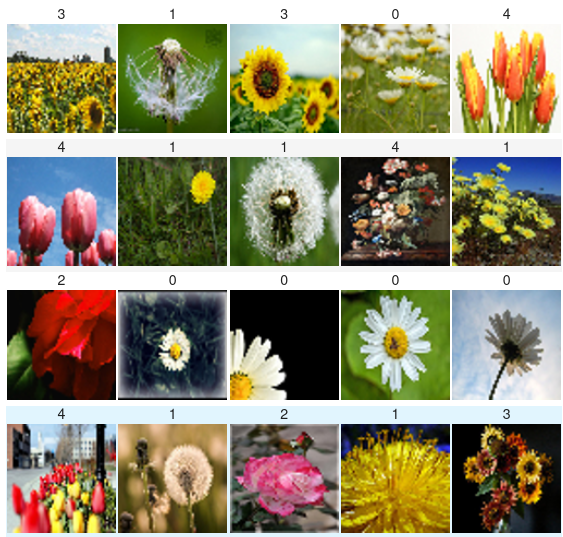
\includegraphics[width=.8\linewidth]{FlowersRan.png} 
\label{fig:wrapfig}
\end{wrapfigure}
\noindent
0-Daisy\\
1-Dandelion\\
2-Rose\\
3-Sunflower\\
4-Tulip\\


Initially, the image data had to be downloaded onto the CS machines in Scratch, and then the images had to be imported themselves. Each image contained a different amount of pixel data, to address this we imported each image to be 56x56 pixels so the network could successfully train on data of the same dimension. During importing, we also created a parallel list with the correct labels added as the images were added to guarantee correct order and labeling to corresponding images. We then normalized these images by diving each pixel value by 255, the range of the image pixel colors, and sorted them into testing and training data to ensure the network was learning to generalize and not just memorize all of the data. We did this by adding 20 percent of the images from each type of flower to testing and the other remaining 80 percent into training. 

\hfill \\

\noindent
The specifics for how the neural network was structured are included below:\\
\hfill \\
\noindent

\includegraphics[width=.5\linewidth]{Prarametrs.png}
\newline
The network contains a total of 928,935 parameters all of which are trainable. This is a significantly higher number of parameters than expected, but we did achieve a decently good accuracy with it. The network has a combination of many convolutional layers of varying sizes to allow the network to recognize features of different sizes and colors, since we made them three dimensional. We also include pooling layers to help the network to minimize the parameter count by lowering the image pixels and forcing the network to combine different portions of the images into one main color of that section. We used dropout layers to try and compensate for the random images that have absolutely nothing to do with the flower data, and then flattening to bring the image into a simpler formatting with fewer parameters. As mentioned, there were random images that were not relevant to the data set, and if it were not so many we would have gone through and manually removed or relabeled the images that were not floral, but there were many images to sort through for that, and it was better to consider the option of additional dropout layers instead.
\newline
The network was trained with 80 percent of each collection of flowers and the test with the 20 percent remaining. Once there was a separation between the training and test data for each flower, the different lists of flowers were combined so all of the training sets for each flower were combined, and same with all of the test sets. 
Both the training and test sets had two lists: a list of images and a parallel list with the answers, both of which had to be shuffled in the same way to guarantee generalization instead of input pattern recognition. 
Training was ended when val accuracy plateaued and loss reached a near zero value. 


\section{Results}

We were able to achieve a val accuracy pf 0.8185, an accuracy of 0.9

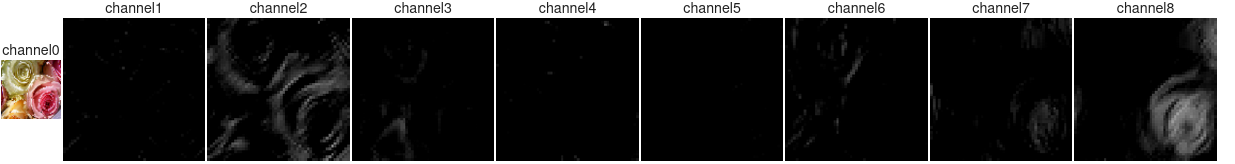
\includegraphics[width=1.2\linewidth]{CHANNELUSE.png}


The following images where taken during training. They show the where the network focused most of its "attention" as it trained on the example image and how the weights percolated up throughout the network. 
\hfill \\

\includegraphics[width=.1\linewidth]{FlowerStack.png}
\includegraphics[width=.1\linewidth]{Flowerstack1.png}
\includegraphics[width=.1\linewidth]{Flowerstack3.png}



\hfill \\
The network was successful in creating feature detectors, as visualized below, and the network appeared to do a pretty good job at locating where the flower was and was often able to distinguish individual petals and a flower center when there was one. \\
\hfill \\

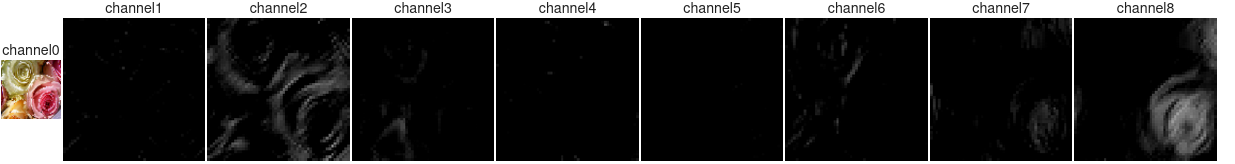
\includegraphics[width=1.0\linewidth]{CHANNELUSE.png} 
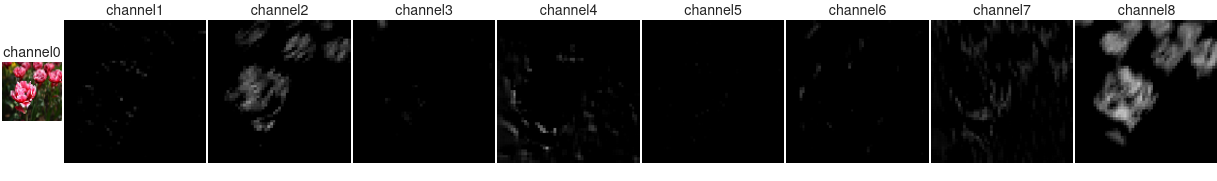
\includegraphics[width=1.0\linewidth]{CHANNELUSE2.png} 
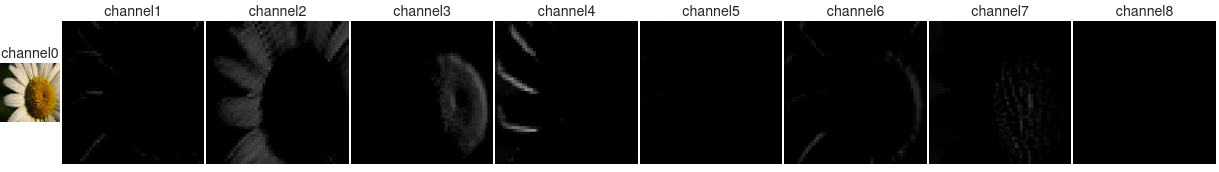
\includegraphics[width=1.0\linewidth]{CHANNELUSE3.png} 
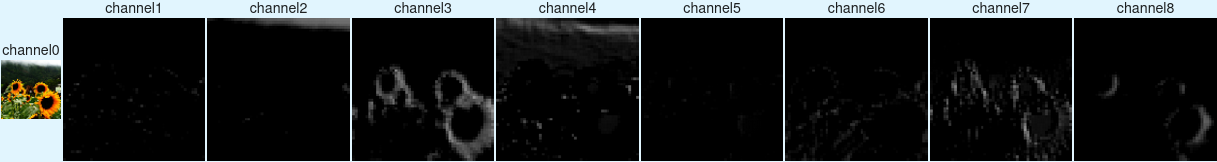
\includegraphics[width=1.0\linewidth]{CHANNELUSE4.png} 
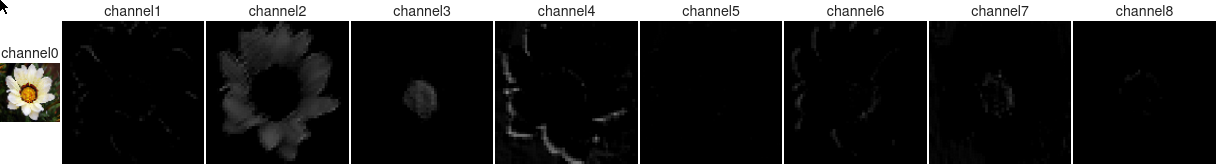
\includegraphics[width=1.0\linewidth]{CHANNELUSE5.png} 
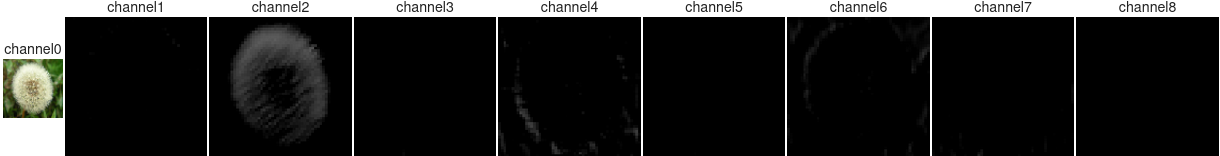
\includegraphics[width=1.0\linewidth]{CHANNELUSE6.png} 
\hfill \\

%Even if your project is not as successful as you'd hoped, you still
%need to show results.  This section is one of the key parts of any
%scientific paper.  Be sure to provide adequate information so that the
%reader can evaluate the outcomes of your experiments. 

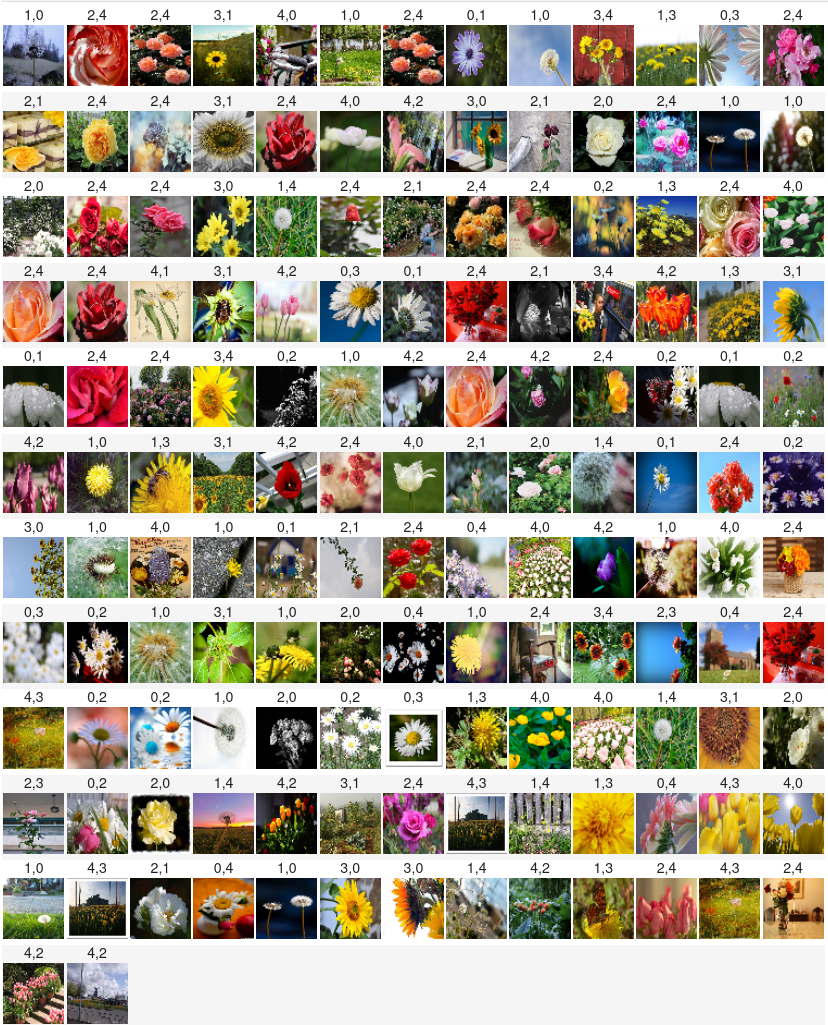
\includegraphics[width=1.0\linewidth]{WRONGUSE.png}


\hfill \\
\hfill \\


\begin{wrapfigure}{l}{0.6\textwidth}
\includegraphics[width=1.\linewidth]{PIEGRAPH.png} 
\label{fig:wrapfig}
\end{wrapfigure}

\section{Conclusions}
While the network was pretty successful, we did not reach the 90 percent accuracy we had wanted, but we are able to see how the different layers detected certain shapes and light levels. We achieved 81 percent accuracy, and while this was below our goal of 90 percent accuracy, we still consider this to be a successful network in that it is still a high percentage, and we acknowledge that 90 percent was a relatively high goal. Some of the error we are encountering we believe to be attributed to some off topic images within the data set, such as the random people who had no flower elements in the images but were included in certain flower folders.

We were able to reach up to 84.5 percent accuracy at distinguishing between the types of flowers given. The most confused types were 

The high error with the network being able to distinguish between a tulip and rose was not surprising to us as they are shaped and colored very similarly. The dandelion and sunflower error was likely due to the fact they have similar coloration, so the light levels would be identified similarly. However the relatively high dandelion to tulip error we did not predict to be an issue, and we are not entirely sure why there is such a high rate of confusion between those two.

\end{document}

\maketitle

\section{Introduction}

\end{document}
